\documentclass[12pt]{report}
\setlength{\parindent}{0pt}
\usepackage{hyperref}
\usepackage{pdfpages}
\begin{document}
% This is the cover letter
\begin{center}
{\bf\huge Requirements specification for Object Creator Team}
\\[3\baselineskip]
{\large Software Engineering (CS240)}
\\[2\baselineskip]
{\large Object Creator team}
\\[2\baselineskip]
{\bf Contributors: }\\
Darren Chu \\ Todd Detweiler \\ Cody Kagawa \\  Lauren Swanson \\  Dongni Wang 
\\[8\baselineskip]
Version 1\\
September 29, 2013 
\end{center} 
\pagebreak

\begin{center}
{\bf\large Abstract \\[1\baselineskip] }
\end{center}
{
\paragraph{\parindent 20pt}This document describes the functions and interactions that occur between the Object Creation module and the various other parties it communicates with in an application called Edith, a collaborative project created by the CS 240 Software Engineering class for fall of 2013. The Object Creation module is responsible for creating sprites, visual representations of objects, to act out the storyline set forth by the user. This document outlines various expected interactions between the module, the user, and other components within Edith, as well as the conditions necessary to properly utilize the software. It also outlines the intended purpose of the module and key design considerations for its construction and use.
}
\pagebreak

{\bf\large Introduction: \\[0\baselineskip] }
\paragraph{\parindent 20pt} Edith will be a web-based version of the instructional system developed at CMU, Alice. It will be a 2D system which allows students to work within a virtual environment in order to create objects and animate them through a story. The objects will be able to be customized by the user through a drag-and-drop interface. Edith will also allow students to use their objects to create animations using a visual programming language, add user interactions to create game-like experiences, and share their creations with others.
\paragraph{\parindent 20pt} We will produce an Object Creator within Edith, which will display a view utilizing the Visual Editor. It will allow the user to create graphical sprites for animations by providing a graphical drawing and manipulation system. The user created sprites will also have user defined behaviors. The objects/sprites will be saved as an output in the form of a JSON specification to be used in other modules.
\paragraph{\parindent 20pt} The Object Creator will serve as a connection between the Visual Editor and the Animation System and allow users to create objects, such as sprites and other story elements, which will be part of a storyline. Graphical representations of the objects will be implemented by the user through painting, manipulating geometrical primitives, or importing images. The user will also be able to define specific behaviors, or methods, for the objects through the use of the Visual Editor. This product will allow the student to switch between the Object Creator and the Story Creator in order to build all the components of their own animation story. The Object Creator will also provide a way for students to use their objects in other modules by saving them in the form of a JSON/Javascript specification of the user defined object. Finally, the Object Creator will run in its own display view, with will include the Visual Editor. 
\paragraph{\parindent 20pt} Edith will be a valuable tool aimed at helping students learn to program through a fun and interactive environment. It will enable students to create their own characters/sprites and animate them throughout a storyline. The users will be able to customize their objects in a drag-and-drop interface and animate those objects through a visual programming language. The students will have the opportunity to add user interactions in order to create game-like experiences and also share their creations with other students. Our Object Creator will work within Edith to provide a way for students to create and manipulate their characters. Our product will serve as a connection between the Animation System, providing necessary tools to create a character, and the Visual Editor, an environment to define character behaviors.

\pagebreak

{\bf\large Use Cases: \\[1\baselineskip] }
Name: Create Object\\
Actor(s): User/Sprite creator
(Sprite creator generates a new sprite for our object, the user specifies parameters of new object)\\
Preconditions/Assumptions: The view has been initialized, file save location specified(not sure if this is part of program start-up sequence)\\[1\baselineskip]
Flow of Events:\\
1. User selects create new object(potentially through interaction with empty space or UI)\\
2. UI prompt generated for user to select between importing or creating image for sprite\\
3. User selects an option and generates image(s) for sprite\\
4. Object creator generates interface for specifying identifiers(name, references, etc)\\
5. User submits name for object\\
6. Images and identifiers converted to JSON/Javascript files and saved into memory.\\
7. Sprite appears on view and sent to story editor(if available)\\
8. Object creation interface disappears\\
9. End of use case\\[1\baselineskip]
Alternatives:\\
- Multiple objects with same name/identifier\\
- File cannot be saved in specified location\\
Postconditions: The object creation interface disappears, new sprite is displayed\\[2\baselineskip]
Name: Create Sprite\\
Actor(s): User\\
Preconditions/Assumptions: The view has been initialized\\

Flow of Events:\\
1. User selects create new sprite option\\
2. Object creator generates new canvas and sprite creator window\\
3. User selects tool from Sprite creator options\\
4. User inputs tool parameters(mouse commands/inputs)\\
5. Input added to canvas\\
6. Repeat actions 3 - 5 as specified by User\\
7. Store canvas data\\
8. Close sprite creator window and send to view\\
9. End of Use Case\\

Postcondition: Sprite creator disappears, sprite is displayed and usable\\[2\baselineskip]

Name: Specify Objects' Names\\
Actor(s): Users/ Sprite creator\\
(Sprite creator can specify the names of the objects. These names would be saved and later be called for adding methods.)\\
Preconditions/Assumptions: Objects have been created\\[1\baselineskip]
Flow of Events: \\
1. User double-clicks the object to select the target.\\
2. User creator right-clicks the screen. Right-click menu will be displayed.\\
3. User left-clicks the "Name" option on the right-click menu.\\
4. A dialog box asking for the user's input within a one-line textbox will be displayed.\\
5.1 If the object hasn't been assigned a name, user can type a name within the textbox.\\
5.2 If the object has had a name, the name will be displayed within the textbox, the user can modify, delete the name or assign a new name for the object.\\
6.1 User clicks the submit button, the object's name will be saved.\\
6.2 User clicks the cancel button, the modification will be canceled. \\
7. End of the use case. \\[1\baselineskip]
Alternatives: \\
-The user has typed illegal characters\\
-The name is too long. (maybe more than 32 letter+numbers)\\
:the input won't be saved, a dialog box would display a warning message. User would have to assign a new name. --back to Event No.4.\\
Postconditions: Methods can be called using the right-click menu.\\[2\baselineskip]
Name: Object Manipulation\\
Actor(s):Users/ Sprite creator\\
(Sprite creator can manipulate the objects. The user can access the Object Manipulations menu and change the object with the specific methods in the menu.)\\
Preconditions/Assumptions: Objects have been created\\[1\baselineskip]
Flow of Events: \\
1. User double-clicks the object to select target\\
2. User right-clicks the object. Right-click menu will be displayed.\\
3. User left-clicks the ?Object Manipulation? option on the right-click menu.\\
4. The Object Manipulation menu will be displayed. \\
5. User left-clicks any of the Object Manipulation options.\\
6. User clicks accept changes once he/she has finished manipulating the object or User clicks cancel changes if he/she wants to undo the manipulations to the object.\\
7. Object Manipulation menu disappears.\\
8. End of Use case.\\[1\baselineskip]
Alternatives:\\
-User moves the object out of the boundaries of the canvas.\\
-User using the Undo or Redo if the object has not been manipulated. \\[1\baselineskip]
Postconditions: The Object Manipulation menu disappears.\\[2\baselineskip]

Name: Importing an image\\
Actor(s): Image importer\\
The user who will be adding the image to the page through importing it.\\
Preconditions: A canvas type layer exists that the image will be imported and displayed on.\\[0\baselineskip]

Flow of Events:\\
1.       Image importer clicks on import image button/option.\\
2.       File reading/uploader window is opened.\\
3.       The importer finds the file on their local machine using the reader window.\\
4.       The image is selected in the reader and sent back to the webpage program.\\
a.       The reader window is closed upon selecting the image.\\
5.        The UI takes the image and creates it as an object on the canvas.\\
a.       The application calls a method to display and create objects sending the method the information on the imported image.\\
6.       The image is displayed in the canvas and saved as a java object with the name of the imported image. \\
7.       End of use case.\\[0\baselineskip]

Alternatives:\\
- The image attempting to be imported is too large for the application to handle. The application throws an error message on the import telling the actor that the image is to large and gives the maximum size allowed (ex: 800x600 pixels). \\
- The name of the imported object is the same name as an object that already exists, in such a case a notification window will pop open letting the user know that a different temporary name has been assigned to the image. \\
- The file was not properly transferred so no import was able to occur.\\
Postcondition:  The image is now displayed in the application canvas and exists as an object to be manipulated.

\pagebreak


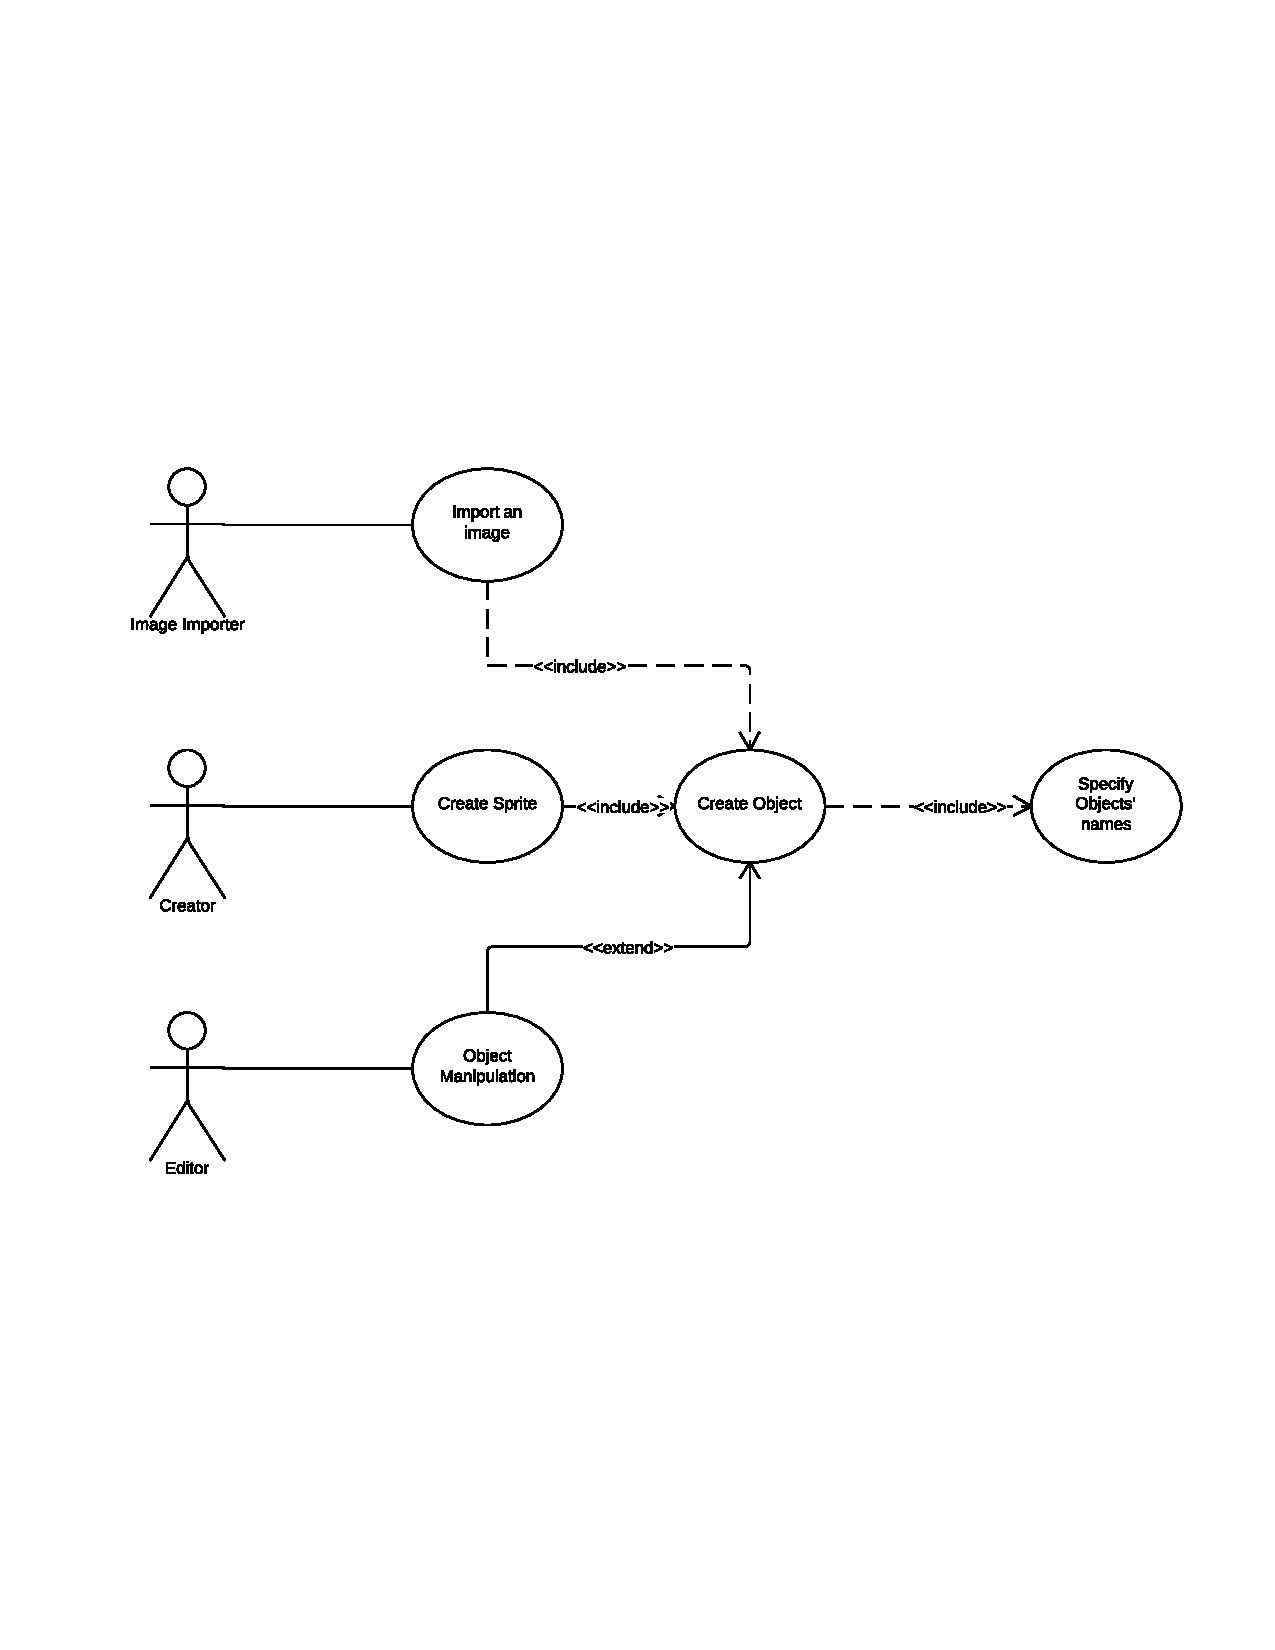
\includepdf[pages={1}]{UML_Diagram.pdf}

{\bf\large Nonfunctional Requirements:}\\[1\baselineskip]
Availability: \\
- The Object-creator module would be available whenever the users log into the system with PC or Macintosh platforms.\\
-The object-creator module should not fail for 90\% of cases.\\[0\baselineskip]

Usability: \\
-The users are not expected to have any knowledge of or previous experience programming.\\
-For users with basic computer operation ability, the average time of learning the facilities of the module independently should be no more than one hour. Ten minutes of training before independent use is possible. \\
-On average, the users with previous experience using graphics editing program may make errors no more than 5 times per hour. The new users may make more errors while learning, but should be able to be skilled users in one hour with informative error messages and well-formed graphical user interfaces.\\[0\baselineskip]

Documentation:\\
-The documentation of object-creator module should be fully understandable to the animation module group.\\
\pagebreak

{\bf\large Glossary/References:}\\[1\baselineskip]
Sprite: object through which the user will be able to define behaviors/actions.
\\[1\baselineskip]
Organizational Requirement Engineering\\
Chapter 9, Non-functional Requirements\\
Prof. Dr. Armin B. Cremers\\
Sascha Alda\\
\url{http://www.iai.uni-bonn.de/III/lehre/vorlesungen/SWT/RE05/slides/09_Non-functional\%20Requirements.pdf}

\end{document}
